\chapter{Практическая часть}

На рисунках \ref{img:example-1} и \ref{img:example-2} представлены примеры работы разработанной программы для описанной СМО без возврата обработанных сообщений и с возвратом.

\begin{figure}[ht!]
	\centering
	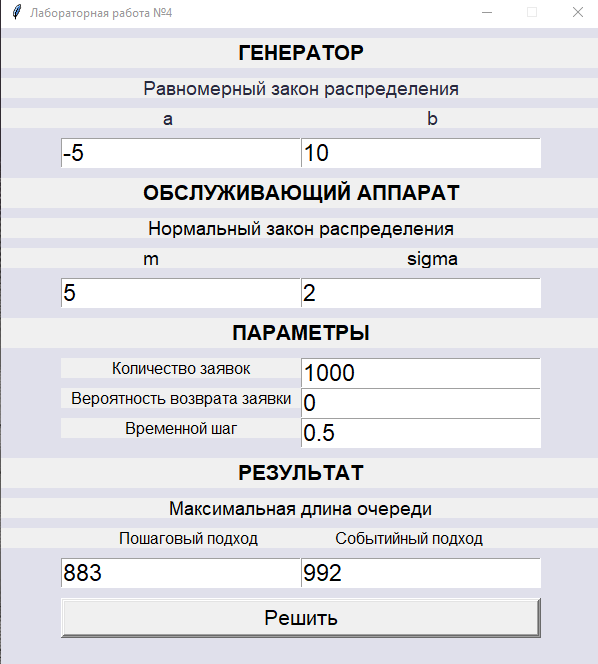
\includegraphics[width=0.6\linewidth]{img/res-1.png}
	\caption{Результат работы программы}
	\label{img:example-1}
\end{figure}

\clearpage

\begin{figure}[ht!]
	\centering
	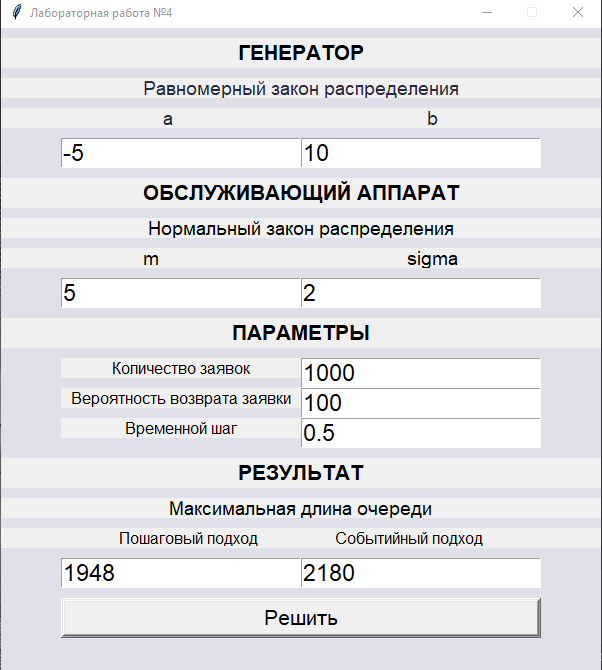
\includegraphics[width=0.6\linewidth]{img/res.png}
	\caption{Результат работы программы}
	\label{img:example-2}
\end{figure}

В ходе выполнения лабораторной работы была реализована программа с графическим интерфейсом для моделирования системы массового обслуживания (СМО) при помощи принципа $\Delta t$ и событийного принципа и определения максимальной длины очереди, при которой не будет потери сообщений. 

